\documentclass[conference]{IEEEtran}
\IEEEoverridecommandlockouts
\usepackage{cite}
\usepackage{amsmath,amssymb,amsfonts,amsthm}
\usepackage{graphicx}
\usepackage{booktabs}
\usepackage{xcolor}
\usepackage[hidelinks]{hyperref}

\newtheorem{theorem}{Theorem}
\newtheorem{proposition}{Proposition}
\newtheorem{corollary}{Corollary}
\newcommand{\ETGE}{\mathbb{E}[T_{\mathrm{GE}}]}
\newcommand{\pres}{P_{\mathrm{res}}}
\DeclareMathOperator{\Prob}{Pr}

\begin{document}

\title{From Gaussian Fading to Gilbert--Elliott:\\ A Closed-Form Bridge for Link-Layer Modeling}

\author{\IEEEauthorblockN{Bhaskar Krishnamachari and Victor Gutierrez}
\IEEEauthorblockA{Viterbi School of Engineering, University of Southern California, Los Angeles, CA, USA\\
Email: \{bkrishna, vagutier\}@usc.edu}}

\maketitle

\begin{abstract}
Correlated Gaussian processes describe dB-domain shadow fading, while Gilbert--Elliott (GE) models provide tractable binary channel abstractions for link-layer analysis. Connecting these representations requires transition probabilities at the time scale sampled by the protocol. We derive closed-form GE parameters that exactly match the one-step conditional probabilities of a thresholded stationary Gaussian process. For arbitrary thresholds, the mapping uses Owen's $T$-function; at the mean threshold, it reduces to a classical arcsine identity. The covariance kernel enters only through the correlation at the sampling lag. This representation yields distinct persistence-time scaling laws: linear growth with the correlation time for the squared-exponential kernel and square-root growth for the exponential kernel at fixed slot duration. We then apply the mapping to truncated ARQ, comparing residual packet loss and throughput with numerically evaluated Gaussian probabilities. In the evaluated setting with three retransmissions, independent losses underestimate residual loss by more than three orders of magnitude and a slot-level GE model misestimates it by up to a factor of 24, whereas a GE model matched directly at the retransmission lag stays within a factor of 1.75. Monte Carlo experiments support the analytical results. The resulting formulas connect physical correlation parameters to link-layer performance and identify the sampling scale needed for useful GE approximations.
\end{abstract}

\begin{IEEEkeywords}
Gilbert--Elliott channel, shadow fading, finite-state Markov channel, burst errors, ARQ.
\end{IEEEkeywords}

\section{Introduction}
Correlated Gaussian processes are widely used to model shadow fading in the dB domain~\cite{gudmundson1991}, while two-state Gilbert--Elliott (GE) models provide a compact description of transmission outcomes~\cite{gilbert1960,elliott1963}. At the link layer, each slot produces either a successful or a failed transmission, and the GE chain captures the temporal memory of this binary sequence. We use the GE chain in its deterministic-output form, in which the observed outcome equals the channel state; this is a special case of the broader Gilbert--Elliott family, whose hidden state need not coincide with the observed error event~\cite{gilbert1960,elliott1963}. GE models are used in ARQ analysis~\cite{zorzi1997,kim1999}; more general FSMCs support queueing analysis~\cite{liu2005}; and intermittent-observation filtering has been studied under independent losses~\cite{sinopoli2004} and GE losses~\cite{wu2018}. GE parameters are often fitted to measured packet-loss or latency traces~\cite{hasslinger2008,nielsen2019} or chosen per scenario.

Finite-state Markov models connect physical fading statistics to discrete channel states through level-crossing approximations and integration of joint fading distributions~\cite{wang1995,zhang1999,sadeghi2008}; ARQ analyses likewise derive Markov transition probabilities from physical channel characteristics~\cite{zorzi1997}. Studies of first-order adequacy further show that model fidelity depends on the channel dynamics, the statistic of interest, and the observation horizon~\cite{wang1996,tan2000,zorzi1995}. For thresholded stationary Gaussian processes, we express the exact one-step transition probabilities directly through the sampled correlation using Owen's $T$-function~\cite{owen1956}. This representation supports both smooth and exponential covariance kernels, yields explicit persistence-time scaling laws, and enables calibration at the retransmission lag.

We derive closed-form GE parameters from the covariance of a stationary Gaussian fading process, characterize their dependence on kernel smoothness, and apply the mapping at the retransmission interval to predict ARQ performance. The contributions are:
\begin{enumerate}
\item \textbf{Closed-form GE parameter mapping.} Closed-form GE transition probabilities that exactly match the one-step conditional statistics of the thresholded Gaussian process, for any stationary covariance kernel (Theorem~\ref{thm:owen}). They reduce to Owen's $T$-function~\cite{owen1956} for general thresholds and to an elementary arcsine identity for the symmetric threshold via Sheppard's classical result~\cite{sheppard1900}.
\item \textbf{Persistence scaling with kernel smoothness.} The GE persistence time $\ETGE$ grows linearly in the correlation time $T_c$ for a smooth (squared-exponential) kernel but only as $\sqrt{T_c}$ for a rough (exponential) kernel. PHY-layer kernel smoothness therefore determines link-layer persistence behavior (Section~\ref{sec:scaling}).
\item \textbf{ARQ prediction at the retransmission interval.} Closed-form residual-loss and throughput predictions for truncated ARQ, evaluated against the Gaussian benchmark. Calibrating the GE chain at the retransmission interval, rather than at the slot interval, substantially improves accuracy (Section~\ref{sec:arq}).
\end{enumerate}
A detailed fidelity analysis of the first-order approximation appears in the full version~\cite{krishnamachari2026} and is summarized in Section~\ref{sec:fidelity}. The code used to produce all results and figures is available at \url{https://github.com/anrgusc/ge-bridge}.

\section{System Model}\label{sec:model}
In wireless propagation, the well-known log-normal shadow-fading model~\cite{gudmundson1991} represents the received signal power in dB as a correlated Gaussian random process. More generally, any fading mechanism whose dB-scale fluctuations are approximately Gaussian and temporally correlated leads to the same mathematical framework. We therefore consider a stationary zero-mean Gaussian process $X(t)$ (representing, e.g., the dB-scale signal power relative to its local mean) with covariance kernel
\begin{equation}\label{eq:sqexp}
K(t,t')=\sigma^2\exp\!\left(-\frac{(t-t')^2}{T_c^2}\right),
\end{equation}
where $\sigma^2$ is the marginal variance (the shadow-fading spread in dB$^2$) and $T_c$ is the correlation time controlling the temporal correlation of the fading process. To explore the effect of kernel smoothness, we also consider the exponential (Ornstein--Uhlenbeck) kernel
\begin{equation}\label{eq:exp}
K_{\exp}(t,t')=\sigma^2\exp\!\left(-\frac{|t-t'|}{T_c}\right),
\end{equation}
which produces a first-order Markov process in continuous time. The exponential kernel is also the Gudmundson shadowing model~\cite{gudmundson1991}, and 3GPP uses the same exponential form for spatial shadowing correlation~\cite[Sec.~7.4.4]{3gpp38901}. For a user moving at constant speed $v$ along a straight line through a spatial shadowing field with decorrelation distance $d_c$, it gives $T_c=d_c/v$. The core derivations below depend on the covariance kernel \emph{only} through the one-slot correlation coefficient $\rho=K(D)/K(0)$, so any stationary Gaussian fading model can be plugged in by computing its own $\rho$ at lag $D$.

Now choose a slot duration $D>0$ and a threshold $S$ (for a fade margin of $F$\,dB, $S=-F$), and sample the process at slot boundaries. Define the binary sequence
\begin{equation}\label{eq:binary}
B(n)=\begin{cases}0, & X(nD)<S,\\ 1, & X(nD)\ge S.\end{cases}
\end{equation}
State 0 denotes an outage (failed transmission), and state 1 denotes a successful transmission. The resulting binary process is not exactly first-order Markov, but it can be approximated by a two-state GE chain with one-step transition probabilities
\begin{align}
p_{01}&=\Prob(B(n{+}1)=1\mid B(n)=0),\nonumber\\
p_{10}&=\Prob(B(n{+}1)=0\mid B(n)=1).\label{eq:pdef}
\end{align}
For the GE abstraction, we define the \emph{GE persistence time} as the expected duration until the next state change when the matched GE chain is observed at a random slot boundary in steady state. If $(\pi_0,\pi_1)$ is the stationary distribution, then
\begin{equation}\label{eq:ETGE}
\ETGE=D\left(\pi_0\frac{1}{p_{01}}+\pi_1\frac{1}{p_{10}}\right).
\end{equation}
This is a statistic of the matched chain; it is determined by the one-step transitions but does not in general equal the remaining duration of the original thresholded process seen from a random slot. For asymmetric thresholds ($S\neq0$), the state-specific dwell times $D/p_{01}$ (mean outage duration) and $D/p_{10}$ (mean time in state 1) are also of interest. Measured from the start of a run, these coincide with the mean run lengths of the thresholded process itself, because in a stationary binary sequence the mean length of 0-runs is $\Prob(B=0)/\Prob(B(n)=0,B(n{+}1)=1)$, which equals $1/p_{01}$.

The distinction concerns how a run is sampled. Measuring from the start of each outage gives equal weight to each outage run. Observing the process at a randomly selected slot instead makes longer runs more likely to be encountered. In the GE chain, geometric run lengths are memoryless, so the expected remaining duration in state 0 is still $D/p_{01}$. The thresholded Gaussian process need not have this property. Thus, matching its mean run lengths does not imply matching its mean remaining duration at a random observation time.

\section{Closed-Form GE Parameters}\label{sec:bridge}
Define $X_0\triangleq X(0)$ and $X_1\triangleq X(D)$. Because $X(t)$ is stationary Gaussian, the pair $(X_0,X_1)$ is jointly Gaussian with zero mean and covariance matrix
\begin{equation}\label{eq:sigma}
\Sigma=\sigma^2\begin{bmatrix}1&\rho\\ \rho&1\end{bmatrix},\qquad \rho\triangleq\frac{K(D)}{K(0)}.
\end{equation}
For the two kernels considered here,
\begin{equation}\label{eq:rho}
\rho_{\mathrm{sqexp}}=e^{-D^2/T_c^2},\qquad \rho_{\exp}=e^{-D/T_c}.
\end{equation}
Normalize by $Z_0=X_0/\sigma$, $Z_1=X_1/\sigma$, $s=S/\sigma$. Let $\Phi(\cdot)$ and $\phi(\cdot)$ denote the standard normal CDF and PDF, and $\Phi_2(a,b;\rho)$ the standard bivariate normal CDF with correlation $\rho$. Then
\begin{equation}\label{eq:p01gen}
p_{01}=\frac{\Prob(Z_0<s,\,Z_1\ge s)}{\Prob(Z_0<s)}=\frac{\Phi(s)-\Phi_2(s,s;\rho)}{\Phi(s)},
\end{equation}
and similarly $p_{10}=\big(\Phi(s)-\Phi_2(s,s;\rho)\big)/\big(1-\Phi(s)\big)$. Introducing the shorthand
\begin{equation}\label{eq:qN}
q\triangleq\Phi(s),\qquad N\triangleq q-\Phi_2(s,s;\rho),
\end{equation}
these become simply $p_{01}=N/q$ and $p_{10}=N/(1-q)$. The GE chain has stationary probabilities $\pi_0=q$ and $\pi_1=1-q$, matching the outage and success probabilities of the thresholded Gaussian process. Substituting into~\eqref{eq:ETGE},
\begin{equation}\label{eq:ETGEclosed}
\ETGE=D\,\frac{\Phi(s)^2+\big(1-\Phi(s)\big)^2}{\Phi(s)-\Phi_2(s,s;\rho)},\qquad \rho=\frac{K(D)}{K(0)}.
\end{equation}
These expressions are \emph{exact} for the one-step conditional probabilities of the thresholded Gaussian process. The matched GE chain therefore preserves the exact one-step binary transitions but not the full higher-order memory (Section~\ref{sec:fidelity}).

The equal-threshold bivariate normal probability admits an exact reduction in terms of Owen's $T$-function~\cite{owen1956},
\begin{equation}\label{eq:owenT}
T(h,a)\triangleq\frac{1}{2\pi}\int_0^a\frac{\exp\!\big(-\tfrac12h^2(1+t^2)\big)}{1+t^2}\,dt,
\end{equation}
which is available in standard numerical libraries (e.g., \texttt{scipy.special.owens\_t}). This yields the main result, stated as a ready-to-use recipe.

\begin{theorem}[GE parameters from Gaussian fading]\label{thm:owen}
Given any stationary Gaussian fading kernel $K$, slot duration $D$, and normalized threshold $s=S/\sigma$, compute $\rho=K(D)/K(0)$ and $a=\sqrt{(1-\rho)/(1+\rho)}$. Then, for any $-1<\rho<1$, $\Phi_2(s,s;\rho)=\Phi(s)-2\,T(s,a)$, so $N=2\,T(s,a)$, and the GE parameters are
\begin{equation}\label{eq:main}
p_{01}=\frac{2\,T(s,a)}{\Phi(s)},\qquad
p_{10}=\frac{2\,T(s,a)}{\Phi(-s)},
\end{equation}
with GE persistence time
\begin{equation}\label{eq:ETGEowen}
\ETGE=D\,\frac{\Phi(s)^2+\big(1-\Phi(s)\big)^2}{2\,T(s,a)}.
\end{equation}
\end{theorem}
\begin{proof}
Owen's identity~\cite{owen1956} for $\Phi_2(h,k;\rho)$, specialized to $h=k=s$, gives $\Phi_2(s,s;\rho)=\Phi(s)-2T(s,a)$ with $a=(1-\rho)/\sqrt{1-\rho^2}=\sqrt{(1-\rho)/(1+\rho)}$. The correction term of the identity vanishes because $hk=s^2\ge0$ and, for $s=0$, $h+k\ge0$. Substituting $N=2T(s,a)$ into $p_{01}=N/q$, $p_{10}=N/(1-q)$ and~\eqref{eq:ETGEclosed} completes the proof.
\end{proof}

\begin{corollary}[Symmetric threshold: arcsine identity]\label{cor:arcsine}
For $S=0$, $T(0,a)=\frac{1}{2\pi}\arctan(a)$, and the identity $\arctan\sqrt{(1-\rho)/(1+\rho)}=\frac{\pi}{4}-\frac12\arcsin\rho$ gives $N=\frac14-\frac{1}{2\pi}\arcsin\rho$. Hence
\begin{equation}\label{eq:arcsine}
p_{01}=p_{10}=\frac12-\frac1\pi\arcsin\rho,\qquad \ETGE=\frac{2D}{1-\frac{2}{\pi}\arcsin\rho}.
\end{equation}
\end{corollary}
Identity~\eqref{eq:arcsine} is Sheppard's classical orthant result~\cite{sheppard1900} expressed as GE transition probabilities. One can verify the limiting behavior directly: when $T_c\to0$, $\rho\to0$ and $p_{01}\to\frac12$ (independent coin flips); when $T_c\to\infty$, $\rho\to1$ and $\ETGE\to\infty$ (frozen channel).

Theorem~\ref{thm:owen} is a one-line computation. Table~\ref{tab:examples} applies it to Gudmundson shadowing with $\sigma=8$\,dB and a fade margin $F=12$\,dB ($s=-1.5$, i.e., $6.7\%$ outage; $|S/\sigma|=1.5$ is also one of the thresholds studied in~\cite{krishnamachari2026}), for LTE-like ($D=1$\,ms) and NR-like ($D=0.125$\,ms) slots.

\emph{Practical operating regime.} Table~\ref{tab:examples} also shows where real links operate. For selected outdoor scenarios, 3GPP specifies shadowing decorrelation distances of $10$/$13$\,m (UMi LOS/NLOS) and $37$/$50$\,m (UMa LOS/NLOS)~\cite[Table~7.5-6]{3gpp38901}. With $d_c=10$--$50$\,m, speeds of $1.5$--$30$\,m/s, and slots of $0.125$--$1$\,ms, $T_c/D=d_c/(vD)$ spans roughly $3\times10^2$ to $3\times10^5$ (about $10^3$--$10^5$ for the scenarios in Table~\ref{tab:examples}), and $1-\rho\approx10^{-5}$--$10^{-3}$. Shadowing is therefore deep in the asymptotic regime of Section~\ref{sec:scaling}. The numerical studies below keep the range $T_c/D\le15$ of~\cite{krishnamachari2026}, where the asymptotes are least accurate and the exact formulas are the ones that matter, and extend to $T_c/D=10^3$--$10^4$ to cover the practical regime.

\begin{table}[t]
\centering
\caption{Theorem~\ref{thm:owen} applied to exponential (Gudmundson) shadowing, $\sigma=8$\,dB, $F=12$\,dB ($s=-1.5$, $\pi_0=0.067$). Speeds and $d_c$ are illustrative values within the range of~\cite[Table~7.5-6]{3gpp38901}.}\label{tab:examples}
\footnotesize
\setlength{\tabcolsep}{2.6pt}
\begin{tabular}{@{}lccccccc@{}}
\toprule
Scenario & $v$ & $d_c$ & $D$ & $1-\rho$ & $p_{10}$ & $p_{01}$ & $D/p_{01}$\\
 & (m/s) & (m) & (ms) & & & & (ms)\\
\midrule
Pedestrian & 1.5 & 20 & 1 & $7.5{\times}10^{-5}$ & $6.8{\times}10^{-4}$ & $9.5{\times}10^{-3}$ & 106\\
 & & & 0.125 & $9.4{\times}10^{-6}$ & $2.4{\times}10^{-4}$ & $3.3{\times}10^{-3}$ & 37\\
Urban & 15 & 20 & 1 & $7.5{\times}10^{-4}$ & $2.1{\times}10^{-3}$ & $3.0{\times}10^{-2}$ & 33\\
 & & & 0.125 & $9.4{\times}10^{-5}$ & $7.6{\times}10^{-4}$ & $1.1{\times}10^{-2}$ & 12\\
Highway & 30 & 50 & 1 & $6.0{\times}10^{-4}$ & $1.9{\times}10^{-3}$ & $2.7{\times}10^{-2}$ & 37\\
 & & & 0.125 & $7.5{\times}10^{-5}$ & $6.8{\times}10^{-4}$ & $9.5{\times}10^{-3}$ & 13\\
\bottomrule
\end{tabular}
\end{table}

\section{Asymptotic Scaling of the GE Persistence Time}\label{sec:scaling}
The key quantity is the one-step threshold-crossing probability $N=\Prob(Z_0<s,\,Z_1\ge s)$. Define $M\triangleq(Z_0+Z_1)/2$ and $\Delta\triangleq Z_1-Z_0$. Because $(Z_0,Z_1)$ is jointly Gaussian and symmetric, $M$ and $\Delta$ are independent Gaussians with $\mathrm{Var}(M)=(1+\rho)/2$ and $\mathrm{Var}(\Delta)=2(1-\rho)$. The crossing event is equivalent to $\Delta\ge0$ and $s-\Delta/2\le M<s+\Delta/2$. When $T_c\gg D$, $\rho\to1$ and the integration window is narrow, so $N\approx\phi(s)\,\mathbb{E}[\Delta_+]$ with $\mathbb{E}[\Delta_+]=\sqrt{(1-\rho)/\pi}$. This yields the following.

\begin{proposition}[Crossing probability asymptotics]\label{prop:asym}
Let $\varepsilon=1-\rho$ and $C(s)\triangleq\sqrt\pi\,\big(\Phi(s)^2+(1-\Phi(s))^2\big)/\phi(s)$. Then $N=\phi(s)\sqrt{\varepsilon/\pi}+O(\varepsilon^{3/2})$, and consequently
\begin{equation}\label{eq:asym}
\ETGE=C(s)\,\frac{D}{\sqrt\varepsilon}+O\!\left(D\sqrt{\varepsilon}\right).
\end{equation}
\end{proposition}

The two kernels therefore give the following scaling laws.

\begin{corollary}[Squared-exponential: linear scaling]\label{cor:se}
For $\rho=e^{-D^2/T_c^2}$, $\varepsilon=D^2/T_c^2+O(D^4/T_c^4)$, and
\begin{equation}\label{eq:linear}
\ETGE=C(s)\,T_c+O(D),\qquad T_c\gg D.
\end{equation}
\end{corollary}
\begin{corollary}[Exponential: square-root scaling]\label{cor:exp}
For $\rho=e^{-D/T_c}$, $\varepsilon=D/T_c+O(D^2/T_c^2)$, and
\begin{equation}\label{eq:sqrt}
\ETGE=C(s)\,\sqrt{DT_c}+O\!\left(\sqrt{D^3/T_c}\right),\qquad T_c\gg D.
\end{equation}
\end{corollary}

\begin{figure}[t]
\centering
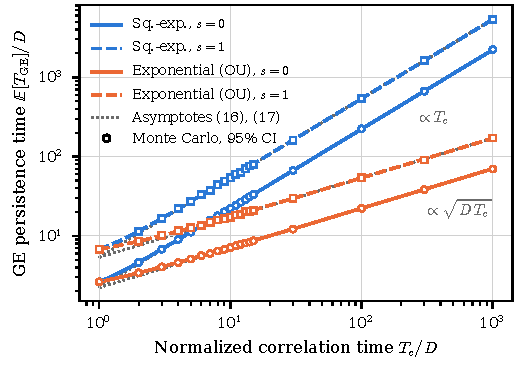
\includegraphics[width=\columnwidth]{fig_scaling.pdf}
\caption{GE persistence time $\ETGE$ versus $T_c/D$ for both kernels and $s\in\{0,1\}$ (symmetric under $s\mapsto-s$). Lines: closed form~\eqref{eq:ETGEowen}. Dotted: asymptotes~\eqref{eq:linear} and~\eqref{eq:sqrt}. Markers: transition probabilities estimated from simulated sequences, inserted into~\eqref{eq:ETGE}, with 95\% CIs.}
\label{fig:scaling}
\end{figure}

\emph{Simulation setup.} The Monte Carlo protocol adapts and extends that of~\cite{krishnamachari2026}, which uses 250 sequences of length 1200 with replication-based confidence intervals. We keep 250 independent sequences per point and length 1200 for $T_c/D\le15$, and extend the length to $200\,T_c/D$ for $T_c/D\in\{30,100,300,1000\}$ so that each sequence contains many fades. Transition probabilities are estimated from transition counts pooled over sequences with a Jeffreys $\tfrac12$ pseudo-count, and 95\% confidence intervals are obtained by bootstrap resampling of sequences.

The qualitative distinction is intuitive. The squared-exponential kernel is infinitely differentiable at the origin, so its sample paths are smooth and the increment $X(D)-X(0)$ is $O(D/T_c)$. The resulting crossing probability scales as $D/T_c$, yielding linear growth of the GE persistence time. The exponential kernel has a cusp at the origin, so its increments are larger, of order $\sqrt{D/T_c}$, and the GE persistence time grows only as $\sqrt{T_c}$. For $S=0$, the linear law also follows in one line from~\eqref{eq:arcsine}: $\arcsin\rho=\frac\pi2-\sqrt{2(1-\rho)}+O((1-\rho)^{3/2})$ gives $\ETGE\approx(\pi/\sqrt2)\,T_c\approx2.22\,T_c$. In the continuous-time limit ($D\to0$), $N/D$ converges to the Rice up-crossing rate $\phi(s)\sqrt{-K''(0)/K(0)}/\sqrt{2\pi}$~\cite[Sec.~3.3]{rice1945} for the smooth kernel; for the exponential kernel $N/D\to\infty$. Fig.~\ref{fig:scaling} confirms both regimes over three decades of $T_c/D$: the transition-count estimates reproduce the analytical GE persistence statistic to within $3.5\%$ at every point, including the practical range $T_c/D\ge100$. At $T_c/D=10^3$ and $s=0$, the two kernels give $\ETGE=2{,}221D$ versus $70D$, a factor of $32$ at the same nominal $T_c$. The asymptotes are already within $0.3\%$ (squared-exponential) and $2.5\%$ (exponential) of the exact values at $T_c/D=10$.

A communications consequence of Corollary~\ref{cor:exp} is that, for exponential (Gudmundson) shadowing, $\ETGE\propto\sqrt{DT_c}$ depends on the slot duration itself. The mean sampled run durations, expressed in physical time, shrink by approximately $\sqrt{8}$ when the slot duration decreases from $1$\,ms to $0.125$\,ms (Table~\ref{tab:examples}). GE parameters must therefore be recomputed for each numerology or TTI. They cannot be inherited from a continuous-time fade-duration formula, because the exponential kernel's level-crossing rate (LCR) is infinite.

\section{Accuracy of the First-Order Markov Approximation}\label{sec:fidelity}
Matching adjacent transitions preserves local binary statistics, but longer runs retain additional dependence. Two diagnostics from~\cite[Sec.~5]{krishnamachari2026} quantify this. The \emph{Markov gap} $\Delta_{\mathrm{gap}}(i,j)\triangleq|\Prob(B_{n+1}{=}1\mid B_n{=}j,B_{n-1}{=}i)-\Prob(B_{n+1}{=}1\mid B_n{=}j)|$ measures how much one additional past slot changes the next-slot prediction. The \emph{run-length total-variation distance} $d_{\mathrm{TV}}$ compares the simulated run-length distribution with the geometric law implied by the GE chain. The two can move in opposite directions: for $S=0$, as $T_c/D$ grows from $2$ to $15$, the squared-exponential kernel's maximum gap falls from $0.096$ to $0.029$ while its $d_{\mathrm{TV}}$ rises from $0.116$ to $0.183$~\cite[Table~1]{krishnamachari2026}. For the exponential kernel, both grow. These diagnostics ask different questions. The Markov gap measures the change in a next-slot prediction when one additional past observation is supplied. The run-length distance measures agreement over entire runs, including their tails. A smaller Markov gap therefore need not imply a closer run-length distribution. Transition-count estimates reproduce the analytical GE persistence statistic, which is a property of the matched chain rather than of the mean residual duration of the thresholded process; the run-length diagnostics reveal additional temporal dependence, with heavier-than-geometric run-length tails at larger $T_c/D$~\cite[Sec.~7.2]{krishnamachari2026}. This distinction matters for ARQ because residual loss depends on a sequence of failed attempts, rather than on a single transition.

\section{Link-Layer Payoff: Truncated ARQ}\label{sec:arq}
We compare a GE chain calibrated at the slot interval with one calibrated directly at the retransmission interval. Consider an ARQ link (or HARQ without soft combining). A packet is first sent in slot $n$. After a failure, it is retransmitted after a round-trip delay of $m$ slots, for at most $L$ retransmissions. Each attempt succeeds if and only if its slot is in state $1$. The \emph{residual loss} is
\begin{equation}
\pres=\Prob\big(B(n)=B(n{+}m)=\dots=B(n{+}Lm)=0\big),
\end{equation}
and the throughput efficiency, defined as successful packets per transmission attempt, is $\eta=(1-\pres)/\mathbb{E}[N_{\rm tx}]$, where $\mathbb{E}[N_{\rm tx}]=\sum_{k=0}^{L}\Prob(\text{first }k\text{ attempts fail})$ is the mean number of transmissions per packet. The denominator counts transmissions, not elapsed time including retransmission waits. Under the Gaussian model, $\pres=\Phi_{L+1}(s\mathbf{1};\mathbf{R})$ with $R_{ij}=K(|i-j|mD)/K(0)$. Here, $\Phi_{L+1}(\cdot;\mathbf{R})$ denotes the standard $(L{+}1)$-variate normal CDF with correlation matrix $\mathbf{R}$, and $\mathbf{1}$ is the all-ones vector. We refer to this as the exact Gaussian model, evaluated numerically: the $(L{+}1)$-dimensional orthant probability is computed with SciPy's implementation of Genz's algorithm~\cite{genz1992} (absolute tolerance $10^{-9}$, relative tolerance $10^{-5}$), and, for the exponential kernel, also by a one-dimensional quadrature recursion, since the lag-$mD$ samples form an AR(1) sequence. It does not, however, yield a design rule in closed form. We compare three closed-form predictors:
\begin{align}
\text{i.i.d.:}\quad &\pres^{\rm iid}=\pi_0^{L+1},\label{eq:iid}\\
\text{Slot-calibrated:}\quad &\pres^{\rm slot}=\pi_0\big[\pi_0+\pi_1\mu^{m}\big]^{L},\label{eq:slot}\\
\text{Lag-calibrated:}\quad &\pres^{\rm lag}=\pi_0\big(1-p^{(m)}_{01}\big)^{L},\label{eq:lag}
\end{align}
where $\pi_0=\Phi(s)$, $\mu=1-p_{01}-p_{10}$, and the bracket in~\eqref{eq:slot} is the $m$-step $0\to0$ probability of the slot-calibrated chain. The quantity $p^{(m)}_{01}$ is Theorem~\ref{thm:owen} evaluated with $\rho_m=K(mD)/K(0)$ in place of $\rho$, i.e., a GE chain calibrated directly at the retransmission interval.

The slot-calibrated model first matches transitions between adjacent slots and then uses $\mathbf{P}^m$, where $\mathbf{P}$ is the slot-calibrated GE transition matrix, to predict outcomes $m$ slots apart. The lag-calibrated model instead matches the two-time Gaussian probabilities at separation $mD$ directly, using the same single evaluation of Owen's $T$-function. The distinction matters because thresholding generally does not preserve the Markov property: an exact adjacent-slot match need not remain exact when the fitted chain is advanced by $m$ steps. Direct lag calibration removes this mismatch for a pair of successive attempts, although predictions involving several attempts still use a first-order approximation.

\begin{figure}[t]
\centering
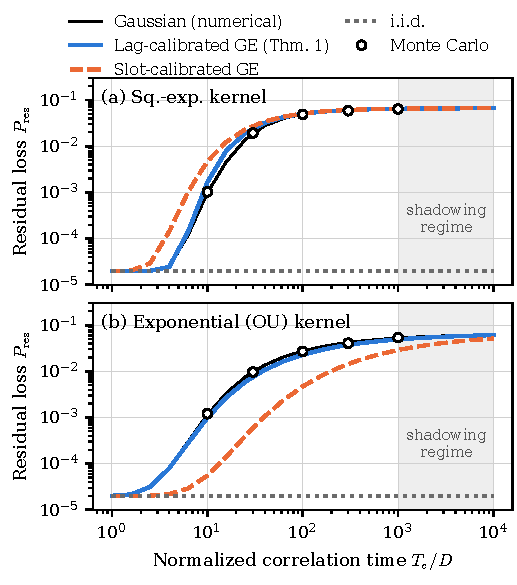
\includegraphics[width=\columnwidth]{fig_arq.pdf}
\caption{Residual loss of truncated ARQ ($s=-1.5$, $m=8$, $L=3$). ``Gaussian (numerical)'' is the exact Gaussian model evaluated numerically~\cite{genz1992}; markers are Monte Carlo (250 sequences of length $\max(4000,200\,T_c/D)$), within $7\%$ of it. Shaded: practical shadowing regime (Table~\ref{tab:examples}).}
\label{fig:arq}
\end{figure}

Fig.~\ref{fig:arq} shows the results for $s=-1.5$ ($6.7\%$ raw outage), $m=8$ and $L=3$, an LTE-like HARQ round trip and retry limit.

\emph{(i) Memory matters by orders of magnitude.} The i.i.d.\ model predicts $\pres=2.0\times10^{-5}$ regardless of mobility. The Gaussian residual loss rises to $0.067$ (squared-exponential) and $0.062$ (exponential), nearly equal to $\pi_0$. In the shadowing regime ($T_c/D\ge10^3$), the i.i.d.\ model is off by more than $2{,}600\times$, because all four attempts fall inside the same fade.

\emph{(ii) The slot-calibrated GE chain is biased, in opposite directions for the two kernels.} Proposition~\ref{prop:asym} applied at lag $mD$ helps explain the exponential-kernel underestimation in the high-correlation limit, for any threshold. The true probability of being in state 1 after $m$ slots, conditional on state 0 now, is $p^{(m)}_{01}\approx\phi(s)\sqrt{\varepsilon_m/\pi}/\Phi(s)$ with $\varepsilon_m=1-\rho_m$. The slot-calibrated chain instead gives $1-[\mathbf{P}^m]_{00}\approx m\,p_{01}\approx m\,\phi(s)\sqrt{\varepsilon/\pi}/\Phi(s)$, valid when $m\,p_{01}\ll1$. For the exponential kernel, $\varepsilon_m\approx m\varepsilon$, so the true $m$-step transition probability grows as $\sqrt m$ while the chain's grows as $m$. This is the $\sqrt{T_c}$ law of Corollary~\ref{cor:exp} reappearing at the protocol scale. The slot-calibrated chain forgets fades too quickly and \emph{underestimates} $\pres$. For the squared-exponential kernel, $\varepsilon_m\approx m^2\varepsilon$, and the two agree to first order when $m\ll T_c/D$. These asymptotics require $T_c/D\gg m$; they do not explain the peak errors or the squared-exponential overestimation at moderate correlation. Numerically, the slot-calibrated chain underestimates $\pres$ by up to $24\times$ for the exponential kernel (at $T_c/D\approx16$), and still by $1.8\times$ at $T_c/D=10^3$. For the squared-exponential kernel, it overestimates $\pres$ by up to $8.6\times$ at $T_c/D\approx6$ before converging for $T_c/D\gtrsim100$.

\emph{(iii) Calibration at the retransmission interval substantially improves agreement.} With three retransmissions and over the full sweep $T_c/D\in[1,10^4]$, the lag-calibrated prediction~\eqref{eq:lag} stays within a factor of $1.75$ of the numerically evaluated Gaussian $\pres$ (relative errors in residual loss from $-21\%$ to $+74\%$), whereas the slot-calibrated chain is off by up to $24\times$ (exponential kernel) and $8.6\times$ (squared-exponential kernel). In the evaluated shadowing regime ($T_c/D\in[10^3,10^4]$), the lag-calibrated prediction is within $7\%$, while the slot-calibrated chain is still off by up to $1.8\times$. The lag-calibrated throughput efficiency $\eta$ is within an absolute difference of $0.008$ of the Gaussian value throughout the evaluated sweep. The i.i.d.\ model instead overstates $\eta$ by up to $0.16$ (e.g., $0.93$ vs.\ $0.80$ for the squared-exponential kernel at $T_c/D=100$).

\begin{table}[t]
\centering
\caption{Minimum retry limit $L$ for $\pres\le 10^{-3}$ ($s=-1.5$, $m=8$).}\label{tab:K}
\footnotesize
\setlength{\tabcolsep}{4pt}
\begin{tabular}{@{}lcccc@{\hskip 8pt}cccc@{}}
\toprule
 & \multicolumn{4}{c}{Sq.-exp.: $T_c/D=$} & \multicolumn{4}{c}{Exponential: $T_c/D=$}\\
\cmidrule(lr){2-5}\cmidrule(lr){6-9}
 & 5 & 10 & 20 & 40 & 5 & 10 & 20 & 40\\
\midrule
i.i.d. & 2 & 2 & 2 & 2 & 2 & 2 & 2 & 2\\
Slot-calibrated GE & 3 & 5 & 10 & 20 & 2 & 2 & 3 & 4\\
Lag-calibrated GE & 2 & 4 & 8 & 18 & 3 & 3 & 5 & 7\\
Gaussian (numerical) & 2 & 3 & 6 & 12 & 3 & 4 & 6 & 9\\
\bottomrule
\end{tabular}
\end{table}

\emph{(iv) Dimensioning the retry limit.} Table~\ref{tab:K} reports the smallest $L$ achieving $\pres\le10^{-3}$ in the moderate-correlation range. The i.i.d.\ model recommends $L=2$ everywhere. For the exponential kernel, the slot-calibrated chain under-provisions ($L=4$ where $9$ is needed at $T_c/D=40$). The lag-calibrated chain also errs on the optimistic side but is within two retransmissions of the Gaussian requirement. For the squared-exponential kernel, both GE models are conservative, reflecting the longer-range dependence discussed in Section~\ref{sec:fidelity}, but the lag-calibrated chain is consistently closer. In the shadowing regime the requirement is much larger: for urban vehicular shadowing ($T_c/D=1333$), even 48 retransmissions ($384$\,ms) leave a residual loss of $1.7\%$ (Gaussian model evaluated by the AR(1) quadrature recursion and confirmed by Monte Carlo), above the $10^{-3}$ target. Meeting such a target at this operating point therefore calls for additional fade margin or diversity rather than more retransmissions. For such long retry chains, the lag-calibrated chain ($9.6\times10^{-4}$) is optimistic by $18\times$, consistent with the heavier-than-geometric run lengths of Section~\ref{sec:fidelity} and with the observation that first-order adequacy depends on the time horizon of the application~\cite{tan2000}; its validated use is the short retry limits typical of HARQ ($L=3$ in Fig.~\ref{fig:arq}).

The model isolates slow fading: it treats each attempt as a threshold test on the shadowing process and ignores small-scale fading, soft combining and link adaptation, all of which would enter through a per-attempt success probability conditioned on $X$. For short retry limits in the evaluated settings, the results support computing GE parameters with Theorem~\ref{thm:owen} at the lag at which the protocol re-samples the channel (here, the HARQ round trip), rather than at the slot interval.

\section{Conclusion}
We derived closed-form GE transition probabilities from the covariance of a stationary Gaussian fading process via Owen's $T$-function, reducing to Sheppard's arcsine identity at the mean threshold. The resulting GE persistence time grows linearly in $T_c$ for the squared-exponential kernel and as $\sqrt{T_c}$ for the exponential kernel, and for Gudmundson shadowing it also depends on the slot duration. For truncated ARQ with three retransmissions, calibrating the GE chain at the retransmission interval keeps residual-loss predictions within a factor of 1.75 of the Gaussian benchmark across the evaluated sweep, and within 7\% in the shadowing regime, whereas a slot-calibrated chain errs by up to a factor of 24 and an independent-loss model by more than three orders of magnitude.

\section*{Acknowledgment}
The development of the mathematical results, code for plots, and writing of this paper have involved the use of AI tools/agents including Claude Code and ChatGPT. The human authors accept full responsibility for its contents.

\bibliographystyle{IEEEtran}
\bibliography{refs}

\end{document}
